%\section{Theoretical Introduction}
\label{sec:cap3}

This chapter presents the theoretical background necessary to understand the techniques and concepts explored in this dissertation. Introduces the reliability challenges of \glspl{fpga} based on \gls{sram}, examines fault-tolerance techniques such as N-Modular Redundancy (NMR) and Dynamic Partial Reconfiguration (DPR), discusses memory scrubbing mechanisms, and outlines the principles of fault injection for resilience evaluation. 

\section{\glsentrytext{fpga}}
This section introduces the \gls{fpga} architecture, focusing on the role of configurable logic blocks, routing resources, and configuration memory.

A \gls{fpga} is a reconfigurable logic device or a programmable \gls{ic} widely used for the implementation of digital systems.

\glspl{fpga} could be reconfigured by the user, even after deployment \cite{Mazzeo2019}. Its programmable nature enables rapid prototyping, hardware acceleration, and long-term design flexibility.

\glspl{fpga} are successful platforms because they combine the flexibility of software with the speed of hardware, providing adaptable computing cores and high-throughput processing of data streams. They are particularly attractive compared to \glspl{asic} due to their shorter development time and costs, and their ability to be reconfigured \cite{8524728}.

\subsection{Core Structure and Components}

An \gls{fpga} is essentially a complex heterogeneous device implemented on a single chip. Its basic structure consists of an array or matrix of interconnected configurable elements:

\subsection{Configurable Logic Blocks}
These are the elementary logic blocks used to implement the desired logic functions. \glspl{clb} (sometimes called Logic Cells or Logic Array Blocks, depending of the \gls{fpga} manufacturer) perform simple combinational and sequential logic.

In the Zynq 7000 \gls{soc}, the \gls{clb} contains a pair of slices, and each of the slices contains four 6-inputs \glspl{lut} and eight storage elements \cite{AMD_UG585}, in the following structure:

These two slices do not have connections between them and are organized by columns, as illustrated in the Figure~\ref{fpga-arch-clb-slice-amd}, and have the following features:

\begin{itemize}
    \item Can be configured as a single 6-input \gls{lut} or two 5-input \glspl{lut};
    \item storage elements (memory capability);
    \item Register (\gls{ff}) and shift register available.
\end{itemize}

A \gls{lut} with $m$ inputs can implement any logical function defined over those $m$ inputs. 
In other words, a 6-input \gls{lut} is capable of performing any Boolean function of up to six variables \cite{Battezzati2010}, \cite{Mazzeo2019}.

The \glspl{lut} could also be configured to other structures:

\begin{itemize}
    \item the so called distributed memory, where each SLICE could be configured as a 64-bit \gls{ram};
    \item 32-bit shift register (SRL32) or two 16-bit (SRL16).
\end{itemize}

\begin{figure}[ht]
\centering
\includegraphics[width=0.75\textwidth]{Cap3/Arrangement-of-Slices-within-the-CLB.png}
\caption{Structure of a \gls{clb} in an AMD7-series \gls{fpga}. Reproduced from \citeauthor{AMD_UG474}}\label{fpga-arch-clb-slice-amd}
\end{figure}

\subsection{Routing and Interconnect Resources}
These resources, including \glspl{sb}, \glspl{cb}, and \glspl{pip}, form a network that electrically interconnects the \glspl{clb}, I/O blocks, and embedded resources to implement complex systems.

\subsection{Input/Output Blocks (IOBs)}
These blocks are positioned around the logic core to interface the internal logic with the external environment, handling data input and output.

\subsection{Specialized Heterogeneous Resources}
Modern FPGAs also include various specialized resources beyond the basic structure, such as:
\begin{itemize}
    \item \textbf{Embedded Memories}, such as \glspl{bram}.
    \item \textbf{Arithmetic Resources}, such as \gls{dsp} units.
    \item \textbf{Processing Resources}, which can be hard cores (e.g., ARM Cortex processors in Xilinx Zynq-7000 \gls{apsoc}) or soft processors implemented using programmable logic.
    \item \textbf{Clock-management resources}.
\end{itemize}

As shown in Figure~\ref{fpga-arch}, the \gls{fpga} architecture consists of configurable logic blocks, routing resources, and \gls{io} blocks.

\begin{figure}[ht]
\centering
\includegraphics[width=0.75\textwidth]{Cap3/fpga-structure.png}
\caption{\gls{fpga} Structure. Adapted from \citeauthor{Marioli2010}}\label{fpga-arch}
\end{figure}

As shown in Figure~\ref{fpga-column-asmbl}, the \gls{fpga} architecture has other specialized hardware, AMD's 7-series is totally based on the columnar approach provided by the \gls{asmbl} architecture. The different domains, represents the diverse platforms with varying feature mixes optimized for different application domains \cite{AMD_UG474}.

\begin{figure}[ht]
\centering
\includegraphics[width=1\textwidth]{Cap3/X30271-ASMBL-Architecture.png}
\caption{\gls{fpga} Structure. Reproduced from \citeauthor{AMD_UG474}}\label{fpga-column-asmbl}
\end{figure}

\subsection{Configuration and Reprogrammability}

FPGAs are programmable devices whose behavior is defined by a \textit{bitstream}. This bitstream contains all the information needed to configure the circuit in the FPGA architecture, mapping the user-defined \gls{hdl} design to the available logic and routing elements.

The type of \gls{cram} used dictates the device's characteristics:

\begin{itemize}
    \item \textbf{\gls{sram}-based \glspl{fpga}:} These are the most widely used commercial FPGAs due to their high reconfiguration flexibility, capability for integrating complex systems, and competitive costs. They use \gls{sram} cells, known as \gls{cram}, to store the configuration. This technology allows FPGAs to be reprogrammed an infinite number of cycles and, crucially, permits \textit{\gls{dpr}}, meaning parts of the configuration can be changed during runtime. A significant drawback is that the \gls{sram} cells are volatile and highly susceptible to radiation-induced faults such as \glspl{seu}, \cite{Adria2023}.

    \item \textbf{Flash-based \glspl{fpga}:} These are reconfigurable and non-volatile, meaning the configuration memory is immune to \glspl{seu}. However, they may have lower capacity and fewer reprogramming cycles compared to SRAM devices \cite{Wubs2023}.

    \item \textbf{Antifuse \glspl{fpga}:} These are One-Time Programmable (OTP) devices whose configuration cannot be changed once set. Their configuration memory is immune to radiation effects, making them suitable for harsh environments, but they offer lower logic capacity \cite{Garcia2020}.
\end{itemize}

\subsubsection{Bitstream}

The bitstream represents the device's configuration for a specific application and is downloaded to the FPGA at startup. Its exact structure and semantics are proprietary and have become increasingly complex over the years.

Several initiatives have attempted to document the structure of the 7‑series bitstream via reverse engineering; a representative example is \cite{f4pga_prjxray}.

Figure~\ref{fpga-simple-bitstream} illustrates, very simplistically, the structure of the bitstream, where we have the header and footer, the sync word and then the \gls{far} that points to one frame \cite{Xilinx_UG470_7Series_Config}.

\begin{figure}[ht]
\centering
\includegraphics[width=0.5\textwidth]{Cap3/simple-bitstream.png}
\caption{Simple representation of the \gls{fpga} bitstream structure.}\label{fpga-simple-bitstream}
\end{figure}

A frame is the smallest unit of configuration data that can be read or written in an \gls{fpga}, identified by a unique 32-bit address divided into five fields: block type, top/bottom position, row address, column address, and minor address \cite{AMD_UG953_IBUF}. Frame addresses are discontinuous due to block cross-distribution, with different blocks corresponding to different frames. These non-contiguous addresses are called physical frame addresses (PFAs), while sequentially arranged PFAs are referred to as linear frame addresses (LFAs) \cite{Xie2023_HybridGrainedScrubbing}. Since bitstream-to-PFA mapping is proprietary, repairing upsets by reconfiguring frames is challenging. Several studies have explored this mapping to infer bitstream structure and address allocation, including \citeauthor{LeRoux2019}, \citeauthor{Aranda2019}, and \citeauthor{Xie2023_HybridGrainedScrubbing}.

A 7-series \gls{fpga} frame consists of 101 words of 32 bits each, where 100 words store configuration data and 1 word contains \gls{ecc} for error correction within the frame.

\section{Sources of Faults in \glsentrytext{fpga}}

Integrated circuits operating in radiation environments are susceptible to transient and permanent faults caused by the interaction of ionizing particles with silicon. Ionizing radiation can generate electrical disturbances by depositing charge that alters transistor states. This deposition occurs either directly, when charged particles interact with the material, or indirectly, when neutral particles such as neutrons produce secondary charged particles (e.g., alpha particles, ions, or protons). The severity of the effect depends on the amount and location of the deposited charge within the semiconductor \cite{KastensmidtRech2016}.

\glspl{see} encompass all radiation-induced phenomena resulting from the interaction of energetic particles with electronic components. These effects are generally classified as hard or soft errors. Hard errors, such as Single Event Burnout (SEB), Single Event Gate Rupture (SEGR), and latch-up (SEL), are permanent and often destructive, while soft errors are recoverable through reset, power cycling, or data rewriting. Among soft errors, Single Event Upsets (SEUs) cause bit flips in memory elements, Multi-Bit Upsets (MBUs) and Multi-Cell Upsets (MCUs) affect multiple storage cells, and Single Event Transients (SETs) induce temporary voltage pulses in analog or combinational logic circuits. In complex integrated systems, Single Event Functional Interrupts (SEFIs) can disrupt control logic or clocks, leading to temporary loss of functionality that typically requires reconfiguration or reset for recovery \cite{Nicolaidis2011}.

Figure~\ref{fig:see_hard_soft} illustrates the classification of the \gls{see} phenomena and their respective subtypes.

%%Types of Errors
\usetikzlibrary{shapes.geometric, arrows}

\tikzstyle{block} = [rectangle, rounded corners, minimum width=4cm, minimum height=1cm, text centered, draw=black, fill=blue!20]
\tikzstyle{subblock} = [rectangle, rounded corners, minimum width=3.5cm, minimum height=0.8cm, text centered, draw=black, fill=green!20]
\tikzstyle{arrow} = [thick,->,>=stealth]

\begin{figure}[ht]
\centering
\begin{adjustbox}{max width=\textwidth}
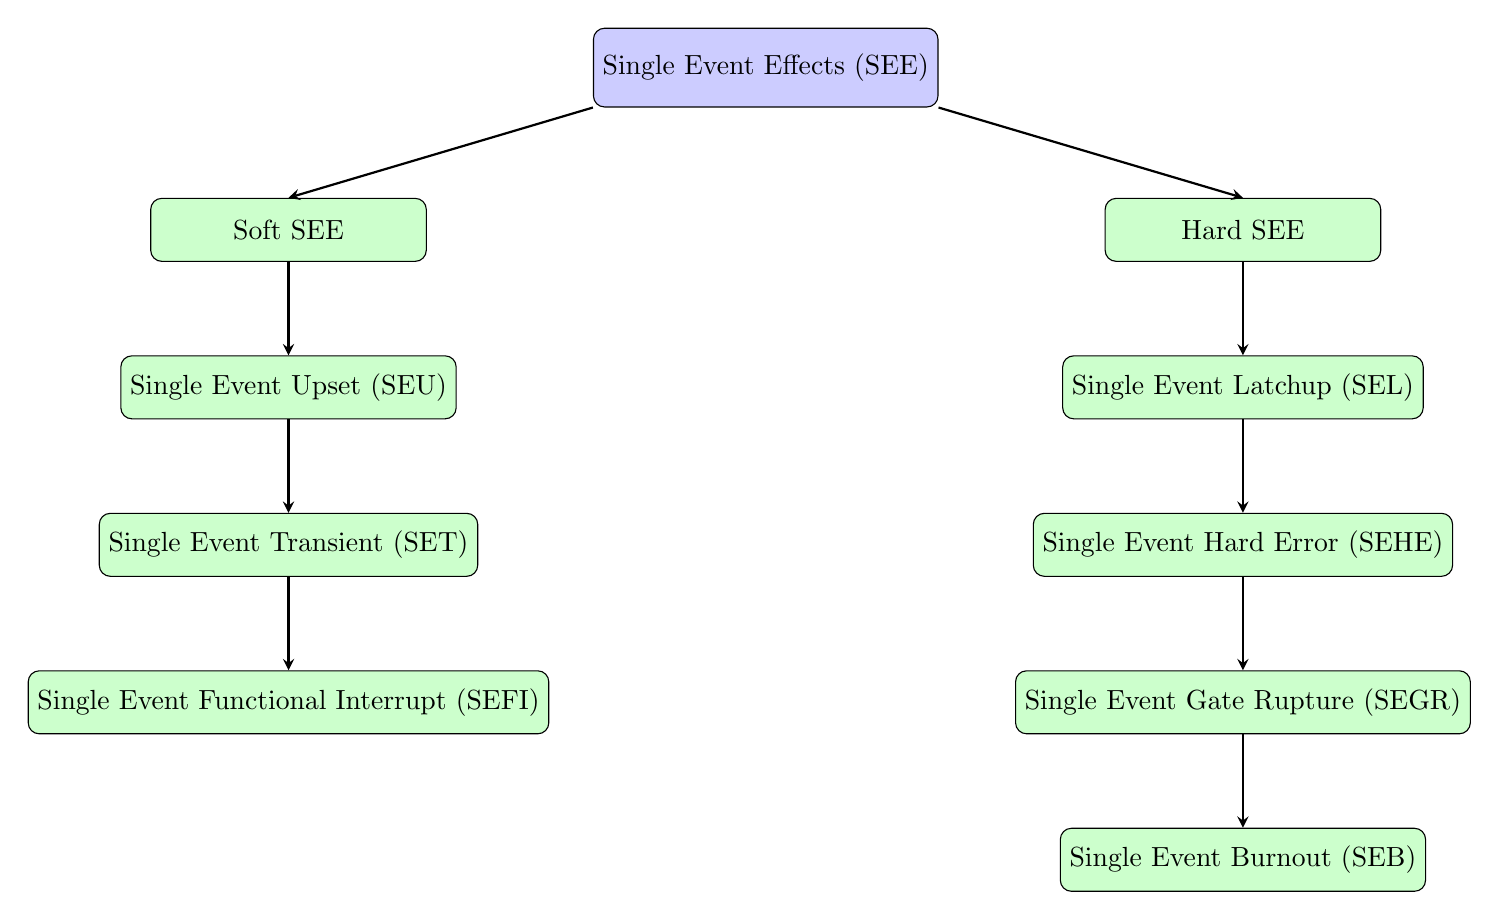
\begin{tikzpicture}[node distance=1.5cm]

% Top-level SEE
\node (see) [block] {Single Event Effects (SEE)};

% Soft SEE
\node (soft) [subblock, below left of=see, xshift=-5cm, yshift=-1cm] {Soft SEE};
\node (seu) [subblock, below of=soft, yshift=-0.5cm] {Single Event Upset (SEU)};
\node (set) [subblock, below of=seu, yshift=-0.5cm] {Single Event Transient (SET)};
\node (sefi_soft) [subblock, below of=set, yshift=-0.5cm] {Single Event Functional Interrupt (SEFI)};

% Hard SEE
\node (hard) [subblock, below right of=see, xshift=5cm, yshift=-1cm] {Hard SEE};
\node (sel) [subblock, below of=hard, yshift=-0.5cm] {Single Event Latchup (SEL)};
\node (sehe) [subblock, below of=sel, yshift=-0.5cm] {Single Event Hard Error (SEHE)};
\node (segr) [subblock, below of=sehe, yshift=-0.5cm] {Single Event Gate Rupture (SEGR)};
\node (seb) [subblock, below of=segr, yshift=-0.5cm] {Single Event Burnout (SEB)};

% Arrows from SEE to Soft and Hard
\draw [arrow] (see.south west) -- (soft.north);
\draw [arrow] (see.south east) -- (hard.north);

% Arrows within Soft SEE
\draw [arrow] (soft.south) -- (seu.north);
\draw [arrow] (seu.south) -- (set.north);
\draw [arrow] (set.south) -- (sefi_soft.north);

% Arrows within Hard SEE
\draw [arrow] (hard.south) -- (sel.north);
\draw [arrow] (sel.south) -- (sehe.north);
\draw [arrow] (sehe.south) -- (segr.north);
\draw [arrow] (segr.south) -- (seb.north);

\end{tikzpicture}
\end{adjustbox}
\caption{Classification of Single Event Effects (SEE) into Soft SEE and Hard SEE with their subtypes.}
\label{fig:see_hard_soft}
\end{figure}

This research focuses exclusively on soft errors, while hard errors are beyond the scope of this study and will not be discussed further.

\subsection{Single Event Upsets (SEUs) and Failure Modes}

Most modern high-density FPGAs rely on \gls{sram} cells to store their configuration bitstream. 

This \gls{cram} defines the functionality of logic blocks (\glspl{lut} and \glspl{ff}) and all internal interconnections. 

Unfortunately, this reliance on volatile SRAM renders FPGAs highly susceptible to soft errors induced by high-energy ionizing radiation, a phenomenon particularly severe in environments such as space.

\subsubsection{Single Event Upsets (SEUs)}

The principal threat to FPGA reliability is the \textit{Single Event Upset (SEU)}, a non-destructive event where a single particle strike flips the state of a memory bit. In \gls{sram}-based FPGAs, \glspl{seu} are a major concern because the altered configuration bits can permanently change the implemented logic and routing, leading to persistent malfunctions, as illustrated in Figures~\ref{fpga-seu-and} and~\ref{fpga-3upsets-cram}.

\subsubsection{\glsentrytext{see} Induced System Failure Types}

When a \gls{seu} hits an essential or critical bit from the \gls{cram} of the \gls{fpga}, it could change the implemented circuit, altering the expected behavior of the affected area.

The change could affect any of the configurable elements of \gls{fpga}, such as the state of the interconnection switches, the clock configuration, the contents of \gls{bram}, the entries in \gls{lut}, or the specific state of the hardware configuration.

Figure~\ref{fpga-seu-and}(a) illustrates one scenario in which a 2-input \gls{lut} is configured by the \gls{cram} bits to describe an $AND$ gate and the \gls{clb} inputs are connected to the inputs $A$ and $B$ by an interconnection switch.

From Table~\ref{tab:logic_gates}, it is evident that the implemented circuit acts as a $AND$ gate, exhibiting the exact behavior described for the values of its inputs.

Then in Figure~\ref{fpga-seu-and}(b), a \gls{seu} is represented, changing the first value of the 2-input \gls{lut} from $0$ to $1$. Now, the behavior of the circuit changes, as shown in Table~\ref{tab:logic_gates}, from a $AND$ gate to an $XNOR$ gate.

Figure~\ref{fpga-seu-and}(c) illustrates another possible scenario, where an interconnection switch is hit by a \gls{seu}, disconnecting the $A$ input from the \gls{lut}. As the input is left floating, the output result is unpredictable. The unconnected input might drift between high or low logic values, depending on nearby static fields. In the worst case, it drifts to an intermediate voltage and only partially switches the output, leading to excess heating of the gate. Or, the output could oscillate between high and low logic values.

\begin{figure}[ht]
\centering
\includegraphics[width=0.75\textwidth]{Cap3/1-s2.0-S014193312300087X-gr1_lrg.jpg}
\caption{FPGA Structure. Adapted from \citeauthor{Mousavi2023_MTTR_FPGA_Scrubbing}}\label{fpga-seu-and}
\end{figure}

\begin{table}[ht!]
\centering
\caption{Truth Tables for AND and XNOR Logic Gates}
\label{tab:logic_gates}
\[
\begin{array}{c c | c @{\hskip 1cm} c c | c}
\multicolumn{3}{c}{\textbf{AND Gate}} & \multicolumn{3}{c}{\textbf{XNOR Gate}} \\
\text{In1} & \text{In2} & \text{Out} & \text{In1} & \text{In2} & \text{Out} \\
\midrule
0 & 0 & 0 & 0 & 0 & 1 \\
0 & 1 & 0 & 0 & 1 & 0 \\
1 & 0 & 0 & 1 & 0 & 0 \\
1 & 1 & 1 & 1 & 1 & 1 \\
\end{array}
\]
\end{table}

\begin{figure}[ht]
\centering
\includegraphics[width=0.75\textwidth]{Cap3/seu-sb-mb.png}
\caption{\gls{sbu} and \gls{mbu} representations in a \gls{fpga} \gls{cram}. Reproduced from \citeauthor{Aguiar2025_SEE_Space_to_Accelerator}}\label{fpga-seu-and-sbu-mbu}
\end{figure}

\begin{figure}[ht]
\centering
\includegraphics[width=0.75\textwidth]{Cap3/fncom-17-1268374-g0001.jpg}
\caption{Representation of different types of upsets in a \gls{fpga} \gls{cram}. Reproduced from \citeauthor{Xie2023_HybridGrainedScrubbing}}\label{fpga-3upsets-cram}
\end{figure}

\section{Reliability Challenges in SRAM-based FPGAs}

SRAM-based FPGAs are widely adopted for their flexibility, performance, and reconfigurability. However, their configuration memory (\gls{cram}) and user logic are highly susceptible to soft errors induced by radiation, electromagnetic interference, or aging effects. These transient faults can alter logic functionality or corrupt stored data, potentially leading to malfunction or complete system failure. Understanding the nature, frequency, and impact of these faults is critical to developing effective mitigation strategies.

The concept of soft error criticality describes the potential of FPGA bits to cause design failures. Upsets in unused regions generally pose a lower risk, as these bits are not expected to affect functionality; however, soft errors could still impact the design if unused elements become inadvertently enabled. Bits configured for the implemented design, whether set to zero or one, are referred to as essential bits. Single-bit upsets in essential bits may be masked by the design, but multiple upsets can accumulate and overcome this inherent protection, potentially leading to errors. Critical bits are those whose flipping can directly cause a system failure, meaning that a single-bit upset in such a bit may compromise the design \cite{Adria2023}. Figure~\ref{fpga-bits-definition} illustrates the classification of the various types of FPGA bits.

\begin{figure}[ht]
\centering
\includegraphics[width=0.75\textwidth]{Cap3/fpga-bits-definition.png}
\caption{Representation of different types of bits in the \gls{fpga} \gls{cram} due to its criticality. Reproduced from \citeauthor{Adria2023}}\label{fpga-bits-definition}
\end{figure}

%%%%%%%%%%%%%%%%%%%%%%%%%%%%%%%%%%%%%%%%%%%%%%%%%%%%%%%%%%%%%%%%%%%%%%%%%%%

\section{N-Modular Redundancy (NMR)}
\gls{nmr} is a fault-masking technique where multiple identical modules operate in parallel, and a majority voter determines the correct output. While \gls{tmr} (Triple Modular Redundancy) is the most common case, extending to higher-order NMR provides increased fault tolerance at the expense of resource overhead. This section explains the mathematical basis of NMR, voter design considerations, fault coverage properties, and limitations regarding permanent resource degradation.

\section{Dynamic Partial Reconfiguration (DPR)}
\gls{dpr} enables the selective reprogramming of specific FPGA regions during runtime without disrupting the operation of unaffected modules. By targeting only the faulty portions of the design, DPR reduces downtime and resource waste compared to full device reprogramming. This section describes the internal mechanisms of DPR, design partitioning strategies, and how it complements redundancy to achieve self-repairing FPGA systems.

\section{Memory Scrubbing Techniques}
Configuration memory scrubbing is a proactive approach that periodically reads and corrects the FPGA configuration to prevent error accumulation. This section discusses different scrubbing approaches, including blind scrubbing, readback-and-verify, and adaptive scrubbing. It also analyzes trade-offs between error coverage, bandwidth consumption, and system availability.

\section{Fault Injection Principles}
Fault injection is an essential method for evaluating the robustness of fault-tolerant FPGA designs. By deliberately introducing controlled errors into the system, researchers can analyze failure modes, verify mitigation strategies, and quantify reliability metrics. This section explains fault injection models (bit-flip, stuck-at), implementation techniques (simulation-based, emulation-based, on-chip), and evaluation criteria.

\section{Fault Injection Overview}

\subsection{Fault Injection Models}
This subsection describes the types of faults that can be injected into FPGA systems. Proper modeling is crucial to evaluate system reliability and test mitigation strategies.

\subsubsection{Bit-Flip Faults}
Bit-flip faults simulate transient errors, such as single-event upsets, in memory cells or configuration bits. These faults are temporary and can occur randomly due to radiation or electromagnetic interference. Studying bit-flip faults helps evaluate the effectiveness of runtime error detection and correction mechanisms.

\subsubsection{Stuck-At Faults}
Stuck-at faults represent permanent logical errors where a signal line is stuck at a logical '0' or '1'. These faults can occur due to manufacturing defects or severe electrical stress. Injecting stuck-at faults allows assessment of system behavior under permanent defects and validates repair mechanisms such as partial dynamic reconfiguration.

\subsection{Implementation Techniques}
This subsection presents the main approaches for performing fault injection in FPGA systems. Each technique has advantages and trade-offs regarding accuracy, speed, and realism.

\subsubsection{Simulation-Based Fault Injection}
Simulation-based techniques introduce faults into software models of the system. This method allows early evaluation without physical hardware and can test a large number of scenarios quickly. However, it may not capture all hardware-specific effects.

\subsubsection{Emulation-Based Fault Injection}
Emulation-based fault injection uses a hardware-in-the-loop setup, often leveraging FPGA prototypes or development boards. This method provides a more accurate assessment than simulation and allows testing of real hardware timing and interactions.

\subsubsection{On-Chip Fault Injection}
On-chip fault injection directly manipulates configuration memory, logic cells, or peripheral interfaces in the FPGA. This approach provides the most realistic evaluation of system behavior under actual fault conditions but may require sophisticated instrumentation and careful safety measures.

\subsection{Evaluation Criteria}
Defining proper evaluation criteria is essential to measure the impact of injected faults and assess mitigation strategies.

\subsubsection{Fault Coverage}
Fault coverage quantifies the proportion of injected faults that are successfully detected or mitigated by the system. High coverage indicates a robust design capable of handling the expected fault rate.

\subsubsection{Error Latency}
Error latency measures the time between fault occurrence and detection or correction. Low latency is critical for systems requiring real-time reliability, such as aerospace or automotive applications.

\subsubsection{Recovery Time}
Recovery time indicates how quickly the system can return to normal operation after a fault. Techniques like NMR, DPR, and memory scrubbing aim to minimize recovery time to maintain continuous operation.


\section{Reliability Metrics and Evaluation Methods}
Assessing the effectiveness of fault-tolerance techniques requires quantitative metrics such as Mean Time Between Failures (MTBF), fault coverage, and error latency. This section introduces these metrics, outlines statistical approaches to evaluate system reliability, and highlights how they guide design trade-offs in FPGA-based systems.

